\documentclass[a4paper,twocolumn]{scrartcl}

\usepackage{graphicx}
%\usepackage{hyperref}
\usepackage{url}
\usepackage{abstract}

%% Limit: 40000 chars
%% check with `detex paper.tex | wc -m`

\title{DNSKEY Management}
\author{Julien Perrochet \and Tobias Schlatter}
\date{December 12, 2012}

\graphicspath{{../figures/}}

\newcommand{\wbjp}{\protect\footnote{Written by Julien Perrochet}}
\newcommand{\wbts}{\protect\footnote{Written by Tobias Schlatter}}


\begin{document}

\twocolumn[
\maketitle
\begin{onecolabstract}
  In this paper we recapitulate the current deployment status of
  DNSSEC and go into the main issues when managing its keys. It
  outlines the paper ``Interadministrative Challenges in Managing
  DNSKEYs'' \cite{Osterweil09} and updates some of its contents
  especially with respect to the signing of the root zone on July
  15, 2012. We will see that DNSSEC penetration in the Internet's
  zones is still low but that the necessary foundations have been lain
  for full deployment.
\end{onecolabstract}
\vspace{\baselineskip}
]



\section{Introduction}
DNSSEC is gradually being deployed in the Internet. However, managing
the cryptographic keys required for the secure delegation provided by
DNSSEC is not always entirely trivial.

In this paper we will first remind of the concepts and operations in
DNSSEC relevant for key management. Then we will give the reader an
overview of the current status of DNSSEC deployment in the Internet to
put the in-detail discussion about key management into the right
context.

Finally, we will shortly outline the DNSSEC situation in Switzerland
(i.e. the \verb|ch.| zone and how its authorities handle DNSKEY management
issues.

\subsection{Chain of Trust\wbjp}
The goal of DNSSEC is to allow resolvers -- any person or process querying a DNS server -- to ensure the authenticity of the reply. Namely, in standard DNS, nothing guarantees the resolvers that his query's answer has not been modified or really originated from a legitimate server.

DNSSEC permits zone operators to \emph{sign} the entries they serve to a resolver, enabling the latter to verify that what he receives is authentic.

This is achieved by establishing a trust chain between something known and the domain that is being queried: e.g., I trust this person to tell me the truth and to be who it claims to be, because a friend I trust is trusting this person.

In the DNS world, the \emph{friend} we trust is the so-called root authority -- the root domain in DNSSEC -- of whom we know the public key in advance.

By signing the keys of the TLD's, the root will put its trust into their keys, and any keys the TLD's have signed, resulting in a trust hierarchy illustrated in fig.~\ref{fig:trust-chain}. This way, a resolver querying the LACAL's DNS server for \verb|lacal.epfl.ch| will be able to verify the received query answer against the known root-authority in the following way:

\begin{enumerate}
\item Verify the reply's authenticity using \verb|lacal.epfl.ch|'s public key, obtained from \verb|epfl.ch|'s DNS server ;
\item Verify the query -- containing \verb|lacal.epfl.ch|'s public key -- returned by \verb|epfl.ch| with its public key, retrieved from the \verb|.ch| DNS server;
\item Again, verify \verb|.ch|'s responses by getting its public key from the root domain.
\item Finally, the root domain's responses can be verified with its already known public key.
\end{enumerate}

DNSSEC's trust hierarchy is similar to the SSL Certificate infrastructure, where an entity marks its trust in another by \emph{signing} its certificate\footnote{Which is nothing more than a public key with additional metadata.}. However, DNSSEC theoretically only has one single top-authority\footnote{The use of TAR's should remain temporary, as in an ideal setup DNSSEC could work without them.}, while the SSL Certificate hierarchy disposes of many.

\begin{figure*}
\center
  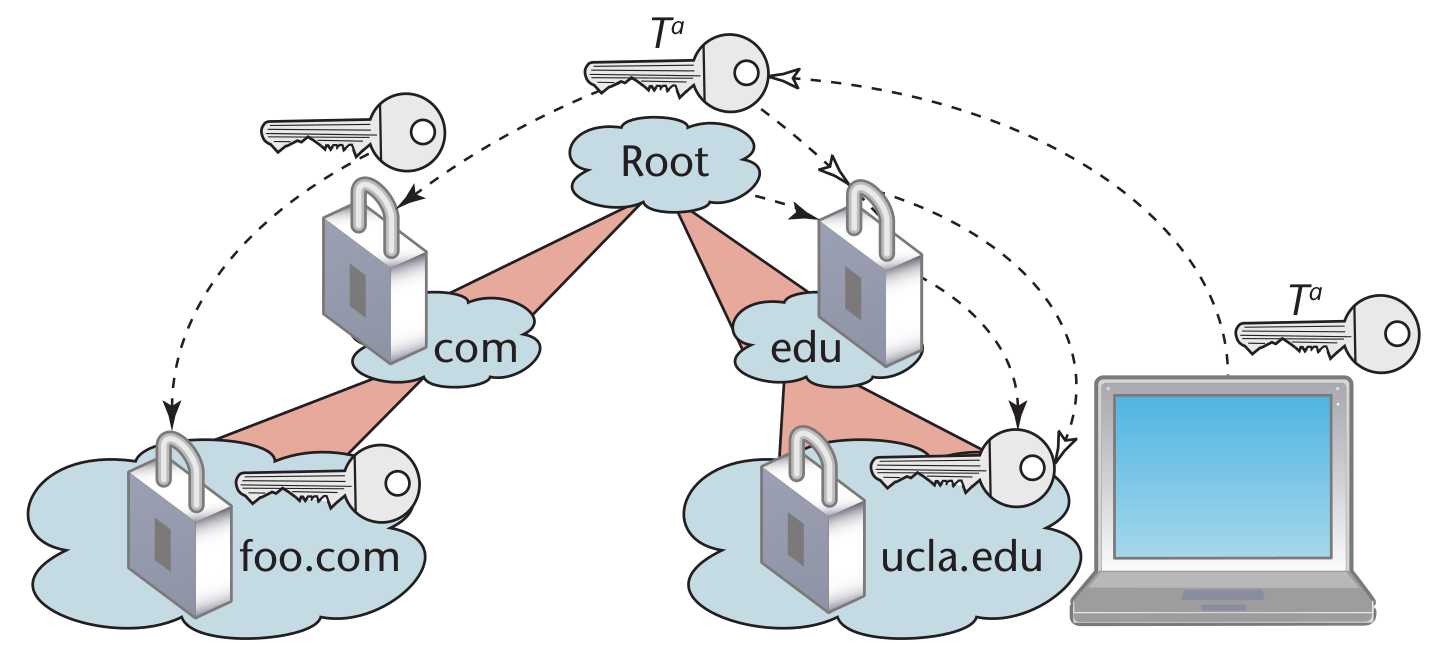
\includegraphics[width=\linewidth]{trust-chain}
  \caption{Example of a trust-hierarchy. Here, the resolver can establish a trust chain between the Root and the ucla.edu zone.}
  \label{fig:trust-chain}
\end{figure*}


 
\subsection{Operations}
In the following, every necessary operation for key management in
DNSSEC is described as a reminder to the reader. This is by no means
intended to give an introduction to DNSSEC but rather to remind the
reader about specific details particularly relevant to this paper.

\paragraph{Enabling DNSSEC} When enabling DNSSEC for a zone, the
parent zone has to establish and sign a DS record with the newly
created public-key.

\paragraph{Key Rollover} RFC4641 \cite{RFC4641} suggests that the DNSKEY
records for a zone should be changed somewhere between once every week
up to once every month. While the detailed rollover procedure is
irrelevant here, it is important to know, that the parent zone has to
update its DS record.

\paragraph{Disabling DNSSEC} An operator might choose to discontinue
DNSSEC for a zone. The DS records (or other means of signing DNSKEYs
as we will see later) need to be removed.

\section{DNSSEC Deployment\wbts}

This section will expose the current deployment status of DNSSEC and
give the reader an idea about the current DNSSEC landscape before
going into the specific DNSKEY management issues. Please refer to
section~\ref{sec:case-study} for more details on the situation of the
\verb|ch.| zone.

\subsection{Penetration in Production}
In figure~\ref{fig:dnssec-growth} you can see the development of
deployed, production DNSSEC zones. The data comes from SecSpider
\cite{secspider} which crawls as many DNSSEC zones as possible,
verifies whether it is properly signed and then applies a heuristics to
determine whether it is actually a production zone. The goal is to
rule out zones which are created for testing such as
\url{bogussig.bogussig.test.jelte.nlnet.labs.nl}.

We can see that DNSSEC is gradually being deployed and the number of
signed production zones grows rapidly (note the log-scale!). The rapid
increase of crawled DNSSEC zones mid-2008, so interprets
\cite{Osterweil09}, is due to a cache poisoning attack discovered in
summer 2008 \cite{dnsVuln}. During our research, we were unfortunately
unable to find an estimate of the number of (production) DNS zones in
the Internet to estimate the percentage of DNSSEC penetration.

Contrary to the state at writing of \cite{Osterweil09}, the DNS
root-zone is signed since July 15, 2010 \cite{root-dnssec} and hence
serves as the global trust anchor. However, as of this writing,
data\footnote{\url{http://secspider.cs.ucla.edu/islands.html}}
gathered by \cite{secspider} suggests that more than half of the
deployed DNSSEC zones which are verifiable (i.e. are likely not to
have a spoofed key, see SecSpider in the next section or
\cite{Osterweil09} for details), do not have a fully linked
certificate chain up to the root zone.

\begin{figure*}
  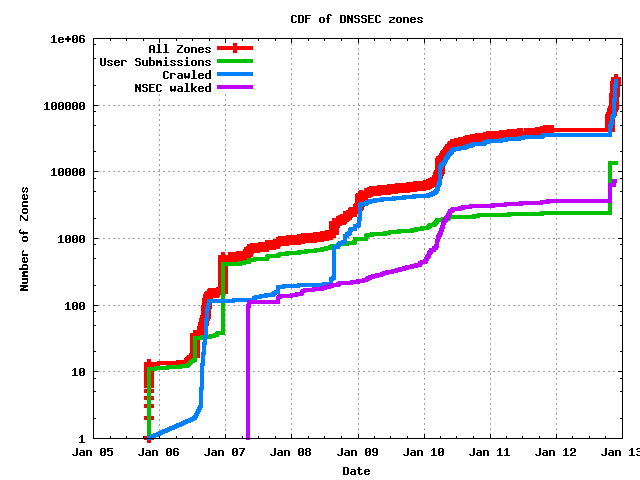
\includegraphics[width=\linewidth]{dnssec-growth}
  \caption{Number of deployed DNSSEC zones by
    SecSpider \cite{secspider}}
  \label{fig:dnssec-growth}
\end{figure*}

\subsection{Trust Anchor Repositories}
Not always can the certificate chain be ensured from the root-zone
down to a DNSSEC zone. Before the signing of the root-zone, it was
obviously impossible to do such a thing, after the signing -- as
formerly discussed data suggests -- there are still orphaned zones
whose parent isn't properly signed.

A Trust Anchor Repository (TAR) can be used in such a situation to
supply resolvers with the trusted public key for a given zone during
DNS resolution, therefore the name \emph{inline repository}. One of
these repositories is the Interim Trust Anchor Repository (ITAR)
formerly operated by IANA and discontinued since the signing of the
root-zone \cite{itar}.

The Internet Software Consortium (ISC) still runs an inline TAR
\cite{iscDlv}, using the DNSSEC Lookaside Validation standard
\cite{RFC5074}. When a resolver needs to check the key of a zone
\verb|<X>| with this TAR, it makes a DNS request of type DLV to 
\url{<X>.dlv.isc.org}. If it succeeds, the DLV record contains the
signature for the (hopefully matching) DNSKEY. The ISC inline TAR
requires manual addition of keys to the repository.

SecSpider \cite{secspider, Osterweil09} is another inline TAR, but
uses a different approach for key validation: Rather then entering and
signing public keys manually, it randomly queries DNSKEY entries from
different point in the world simultaneously and only enters it into
the TAR, if all the received keys match. This makes spoofing of a key
very difficult due to the spatial distribution and the
unpredictability of the queries.

Another type of TAR resides at the resolver: A statically configured
TAR stores keys locally at the resolver and hence needs not to issue an
additional query for keys when a new DNS request arrives. The
statically configured TAR may automatically poll keys asynchronously,
or is maybe just a bunch of manually configured trusted keys. As an
example of a statically configured TAR, we have
Vantages\footnote{\url{http://www.vantage-points.org/}}, an addition
to a standard resolver, \cite{Osterweil09} which can poll keys from
different locations such as web pages, but also also other
vantage-enabled resolvers. Of course, the operator may also choose to
add trusted keys manually.

\section{Operations\wbjp}
This section covers the issues and quirks related to the management of DNSSEC.
\subsection{3Rs}
%% Talk about EPP or push burden to Case-Study
Regarding the management of the Internet namespace, three entities can generally be considered:

\begin{itemize}
\item a registry;
\item a registrant;
\item a registrar.
\end{itemize}

The registries are the entities serving the records for a zone. For example, Switch is the registry for the \verb|ch.| zone. Registrants, on their side, are the entities willing to obtain a certain domain: the registrant of \verb|epfl.ch| is the school in itself (its IT-department to be precise \footnote{As a \emph{whois} query on the epfl.ch domain will show you.}), for example.

These two entities can eventually be linked by the third one, the registrar: this is where registrants will obtain the actual registration service, namely, the linking between a domain name and an IP address.

In Switzerland, for example, Switch plays both the roles of the registry and a registrar: other registrars also exist but one can purchase a domain name directly from Switch. Registries will generally delegate part or whole of the namespace registration managing to registrars\footnote{For example, one can also buy a .ch domain from \url{http://gandi.net}}

Registrants are also free to play the registry and registrar roles for their own sub-domains: groups, laboratories and associations within EPFL may apply for an \verb|epfl.ch| sub-domain, like the LACAL and it's \verb|lacal.epfl.ch| subdomain, for example.

The entities behind the three R's are the exact same whether DNSSEC is used or not, but DNSSEC modifies the relations among them: e.g., DNSKEY updates will now also require communication between the three R's, even if no practical information like IP addresses or billing data was actually updated.

\subsection{Signing a zone}
Whenever an entity wishes to sign its zone, it should ideally turn to its already signed parent zone, in order to create a continuous trust chain.
Said parent should then serve a DS record containing the child zone's key signature.

Signing new zones will have different administrative implications depending on whether the parent zone is in the same administrative entity or not: e.g., \verb|www.epfl.ch| is managed by the same entity as \verb|epfl.ch|, so signing the \verb|www| sub-domain will imply a different (and very likely easier) procedure than signing \verb|epfl.ae|, EPFL's domain for its middle-east campus.

\subsubsection{Single administrative domain}
Basically, once an organization has its main domain signed, it is relatively easy for any sub-entity within said organization to get a sub-domain signed, and to coordinate any operations relative to DNSSEC like key rollover: staying with our EPFL example, it can suffice to contact the IT-department and discuss about the procedure with them\footnote{EPFL does not actually use DNSSEC, but we use the school as an example for the sake of simplicity.}. The bottom line is that it is relatively easy to handle the additional work and information updates required by DNSSEC as long as every concerned party lies within the same organization.
\subsubsection{Multiple administrative domain}
DNSSEC's true challenges arise when we begin to consider several administrative entities (the three R's, mainly). As stated earlier, once the \verb|epfl.ch| zone is signed it is easy for the school to sign \verb|www.epfl.ch|. However, if the domain to be signed was \verb|epfl.ch| or \verb|epfl.ae|, the school would have to deal with the entity or entities managing the TLD's (\verb|ch.| managed by Switch or \verb|ae.|\footnote{epfl.ae has been registered at 'Instra Corporation Pty Ltd', a registrar for the ae.}, respectively), which will have they own terms and conditions, which might very well be different among different registrars and TLD's. 	

While standard DNS can perfectly live with some of the temporary imprecisions generated by non-optimal interactions between the three R's, DNSSEC is far less tolerant to such jitter: typically, if the \verb|epfl.ch| zone updates its keys but Switch fails to reflect this change fast enough in its records, query responses from \verb|epfl.ch|'s DNS servers will appear as illegitimate whereas they perfectly are, and this will last as long as Switch's servers do not reflect the update.

As suggested by some RFC\footnote{RFC 4641}, key updates should  happen at least every few months. Hence, it is crucial that a streamlined and reactive process is available for child-zones to notify their parent-zone when required. In the three R's setup, this means that the registry (or the registrars) must provide means for registrants to easily inform them of any changes regarding their DNSSEC keys.
%TODO process figure with Registrant -> Registrar -> Registry ?


Furthermore, as these communications concern the DNSSEC setup, security must be guaranteed: if a registry's update tools allow an attacker to update the key signatures, the whole point of DNSSEC is moot.

\paragraph*{Entity Roles Overlap} Another issue arises when we consider the fact that registrants may outsource part or whole of the hosting burden, like:

\begin{description}
\item[Key Signing] Services that will handle the zone signing and key rollovers are available\footnote{like this registrar: \url{http://registrars.nominet.org.uk/registration-and-domain-management/dns/dnssec-signing-service}}.
\item[Hosting] Countless hosting services are available, many of which are proposed by actual registrars. Some of them can also propose DNSSEC to their customers, in addition to the standard DNS service they also provide.
\end{description}

While having the registrars also handle DNSSEC will ease managing key rollovers and updates, it creates another problem: registrants, who generally are the registrars or registry's customers, might very well decide to switch from one service provider to another.

If standard DNS simply provides zone transfers as a mean enabling such migrations, DNSSEC must be treated differently. Whether a new private-public key pair is generated or whether the existing pair is transferred, new hurdles are introduced:

\begin{itemize}
\item[-] The transferred private key is not totally \emph{private} anymore, as now both the old and new service provider know it;
\item[-] Newly generated keys will require an update of the parent zone, and this might happen outside of normally planned rollover periods.
\end{itemize}

Another issue is that hosting and key signing services that are not registrars don't have to comply to any of ICANN's rules, increasing the difficulty to enforce common procedures, as none of these services is contractually bound to do so.

\subsection{Computing power}
DNSSEC does not only require a higher coordination among the three R's, it also increases the strain on the computing infrastructure of a registrar when the size and quantity of the  zones it manages grow: updates to a zone or key rollovers require cryptographic signing operations that are orders of magnitude more expensive than simply updating the DNS record. Even with improvements like incremental signing, the computational requirements are significant and must be considered when a registrar whishes to enable DNSSEC.
%TODO find good ref on this.

\subsection{Disabling DNSSEC}
The final and somewhat unintuitive managerial issue with DNSSEC is what needs to be done once a zone administrator wishes to turn it off. 

In such a case, it is absolutely insufficient to only disable the service on the devices serving the aforementioned  zone: in doing so, resolvers won't be able to distinguish between spoofed DNS replies that contain non-DNSSEC data and legitimate replies that simply stopped using DNSSEC.

For DNSSEC's shutdown to be clean and complete, the parent zone and any TAR must be cleaned from whatever DS record they contain for the zone which is being withdrawn from DNSSEC.

Again, this teardown must happen in a synchronous way -- requiring additional effort with regard to DNS -- as resolvers will perceive the domain to be \emph{broken} as long as all involved parties are in a incoherent state.


\section{Case-Study: \texttt{ch.} Zone\wbts}
\label{sec:case-study}

The \verb|ch.| zone is managed by SWITCH, the institution which also
employs the Swiss educational network. In this section we briefly
point out the current deployment status of DNSSEC and how SWITCH
handles the discussed key management issues.

\paragraph{Certificate Chain} According to a query on SecSpider
\cite{secspider}, the \verb|ch.| TLD zone is signed and fully
verifiable from the root zone anchor on downwards. The certificate
chain can hence fully be established and no separate TAR is required.

\paragraph{Penetration} SWITCH states on their website that as of
30. September 2012, 1'734'170 child-zones of \verb|ch.| have been
registered\footnote{\url{https://www.nic.ch/reg/cm/wcm-page/statistics/index.html}}. Upon
inquiry, SWITCH stated that there are around 370 secure delegations
from the \verb|ch.| zone. This is less than $0.02\%$ penetration
rate.

\paragraph{Key Management} The validity period of a zone signing key
(for \verb|ch.|) is 37 days \cite{switch10}. For child zones,  DNSSEC
and DNSKEY entries can be enabled and disabled through SWITCH's 
web-interface which is able to pull the keys automatically from the
authoritative DNS servers. Partners (as Registrars are called in
Switzerland) may also use EPP for key rollover.

Therefore, it is relatively simple to enable DNSSEC for a \verb|<X>.ch.| 
zone. While using the web-interface is certainly cumbersome when
having to deal with rollovers for a large number of domains, any major
provider may become a SWITCH Partner and can then switch over to EPP
which solves this issue.

\paragraph{Cost} DNSSEC secure delegation is currently provided by
SWITCH with no additional cost to normal DNS delegation.

\nocite{*}
\bibliographystyle{abbrv}
\bibliography{dnssec}

\end{document}

%%% Local Variables: 
%%% mode: latex
%%% TeX-master: t
%%% End: 
